
\section{Цель работы}
\begin{frame}\frametitle{Цель работы}
    \large \textbf{Цель работы - Получение и измерение параметров установки высокого вакуума}  
    
    \large{\\ В работе используются: Вакуумная установка с манометрами: масляным, термопарным, ионизационным.}\\
    \begin{itemize}
        \large \normalsize{}
    \end{itemize}
\end{frame}


\begin{frame}\frametitle{Установка}
    \begin{figure}
        \centering
        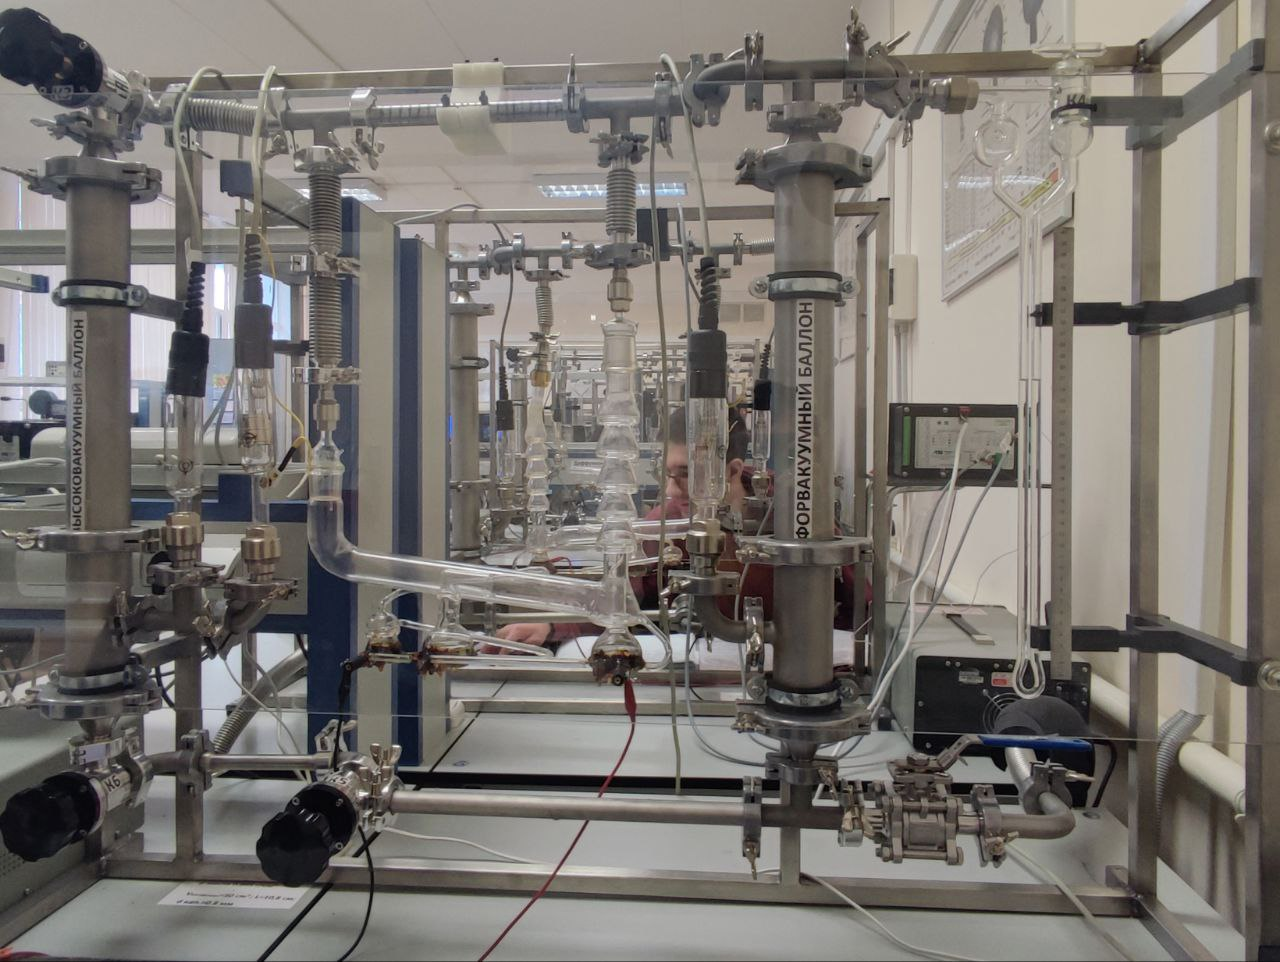
\includegraphics[scale=0.2]{images/full.jpg}
        \caption{1. Полная фотография установки}
        \label{fig:my_label}
    \end{figure}
\end{frame}


\begin{frame}\frametitle{Ход работы: определение объёмов}
    Изначально все краны открыты, в установке находится атмосферный воздух. Далее закрываются краны \textbf{5} и \textbf{6} и включается форвакуумный насос, объём запертого в перемычке между ними воздуха \(V_1 = 50 \text{ см}^3\)
    \begin{figure}
        \centering
        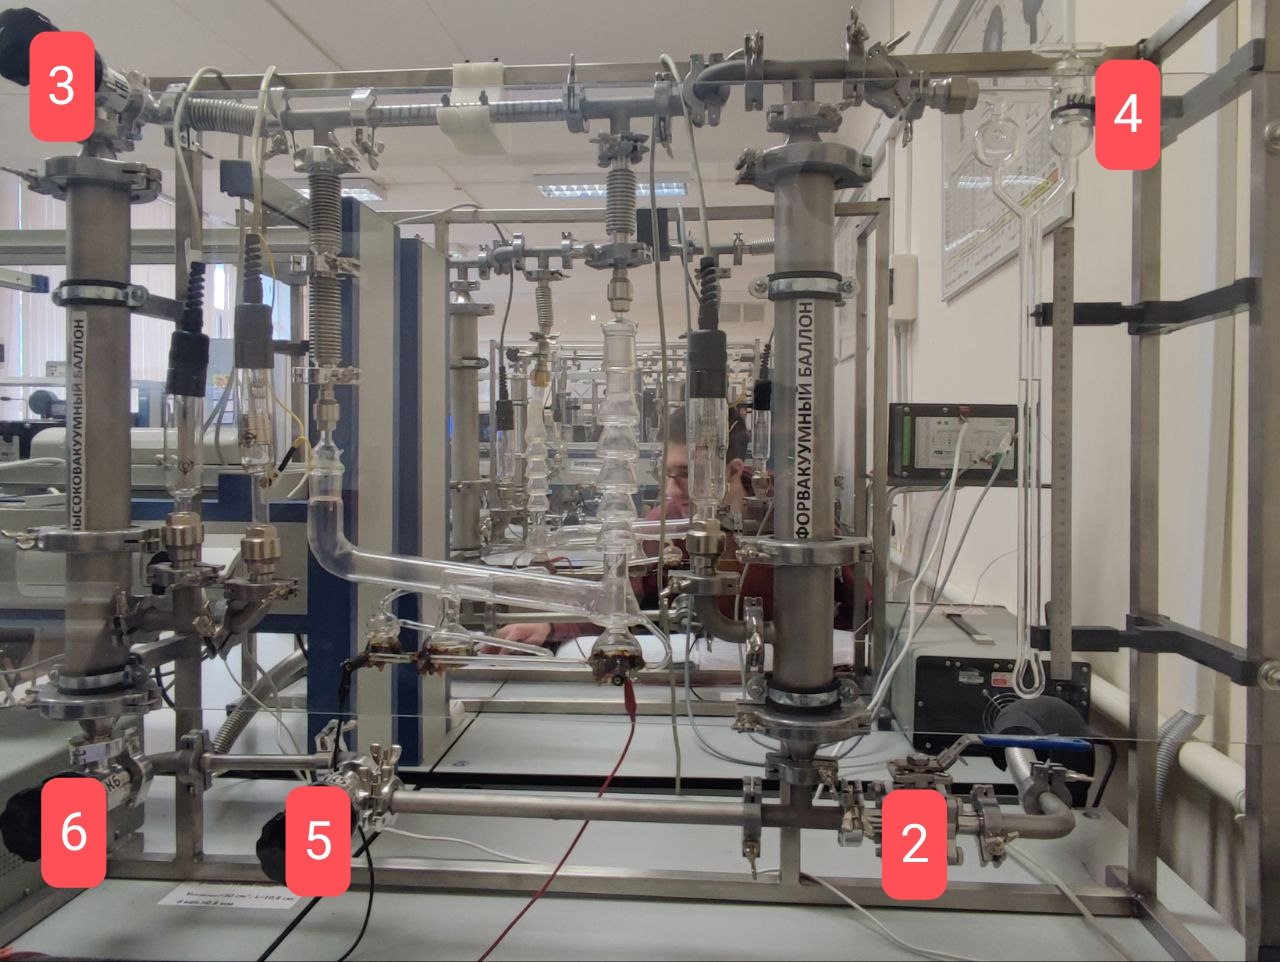
\includegraphics[scale=0.19]{images/valve.jpg}
    \end{figure}
\end{frame}


\begin{frame}{Ход работы: определение объёмов}
    По достижении \(p_{c0} \approx 10^{-2}\) мм.рт.столба закрываем \textbf{2} и \textbf{4} краны, форвакуумный насос работает. Манометр уже готов к работе, в его правом колене вакуум. 
    \begin{figure}
        \centering
        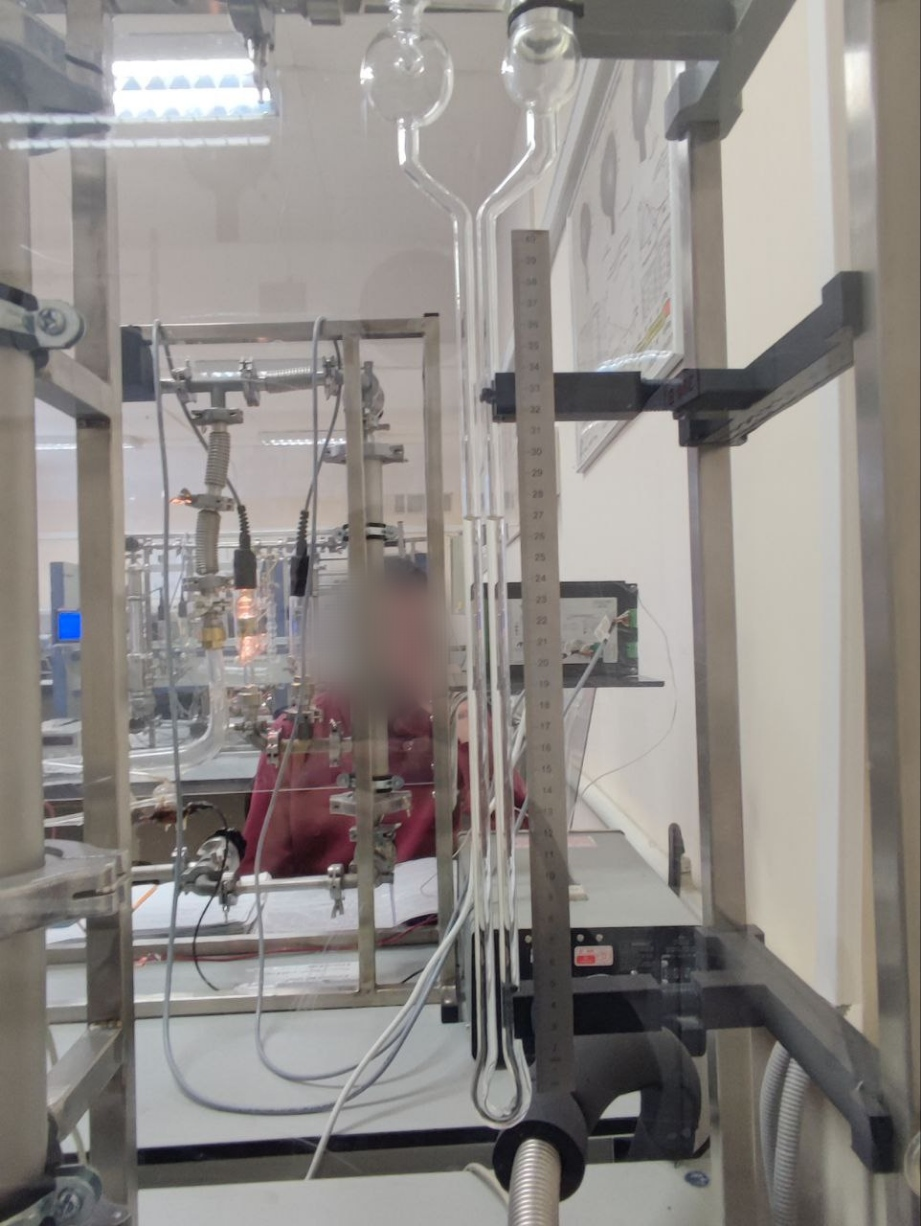
\includegraphics[scale=0.15]{images/oil_manometer.jpg}
    \end{figure}
\end{frame}


\begin{frame}{Ход работы: определение объёмов}
Далее закрывается \textbf{3} кран, отделяющий форвакуумную часть от высоковакуумного баллона. Масляный манометр показывает высоты (см.масл.столб)
\begin{table}[h!]
\begin{tabular}{|c |c|}
\hline
h_{up} & h_{down} \\
\hline
39.9  \pm 0.1     & 12.9 \pm 0.1 \\    
\hline
\end{tabular}
\end{table}
Что дает давление: 
$p_1= 27.0 \pm 0.2\text{ см.масл.столба} = 17.36 \pm  0.13\text{ мм.рт.столба} $

Откуда объем форвакуумной части (\(T = T_{room}\)) \(V_f=V_0\frac{p_0}{p_1}= 2.88 \pm 5 \cdot 10^{-2} \text{ л}\)

\end{frame}


\begin{frame}{Ход работы: определение объёмов}
    Далее открывается высоковакуумный баллон, и манометр показывает \\ \begin{table}[h!]
\begin{tabular}{|c |c |}
\hline
h_{up} & h_{down} \\
\hline
35.3 \pm 0.1     & 18.3 \pm 0.1  \\
\hline
\end{tabular}
\end{table}
Откуда давление в системе: 
$p_2=\rho g (h_1-h_2) = 17.0 \pm 0.2 \text{ см.масл.столб}$

И объем баллона \(V_h=V_f(\frac{p1}{p2}-1)= 1.82 \pm 5 \cdot 10^{-2} \text{ л}\)
\end{frame}


\begin{frame}{Ход работы: создание высокого вакуума}
    После измерения объёмов открываем \textbf{все} краны, откачиваем воздух. \\
    Проводим измерение давления в высоковакуумной и форвакуумной частях при помощи термопарных манометров.
    \begin{figure}[h]
        \centering
        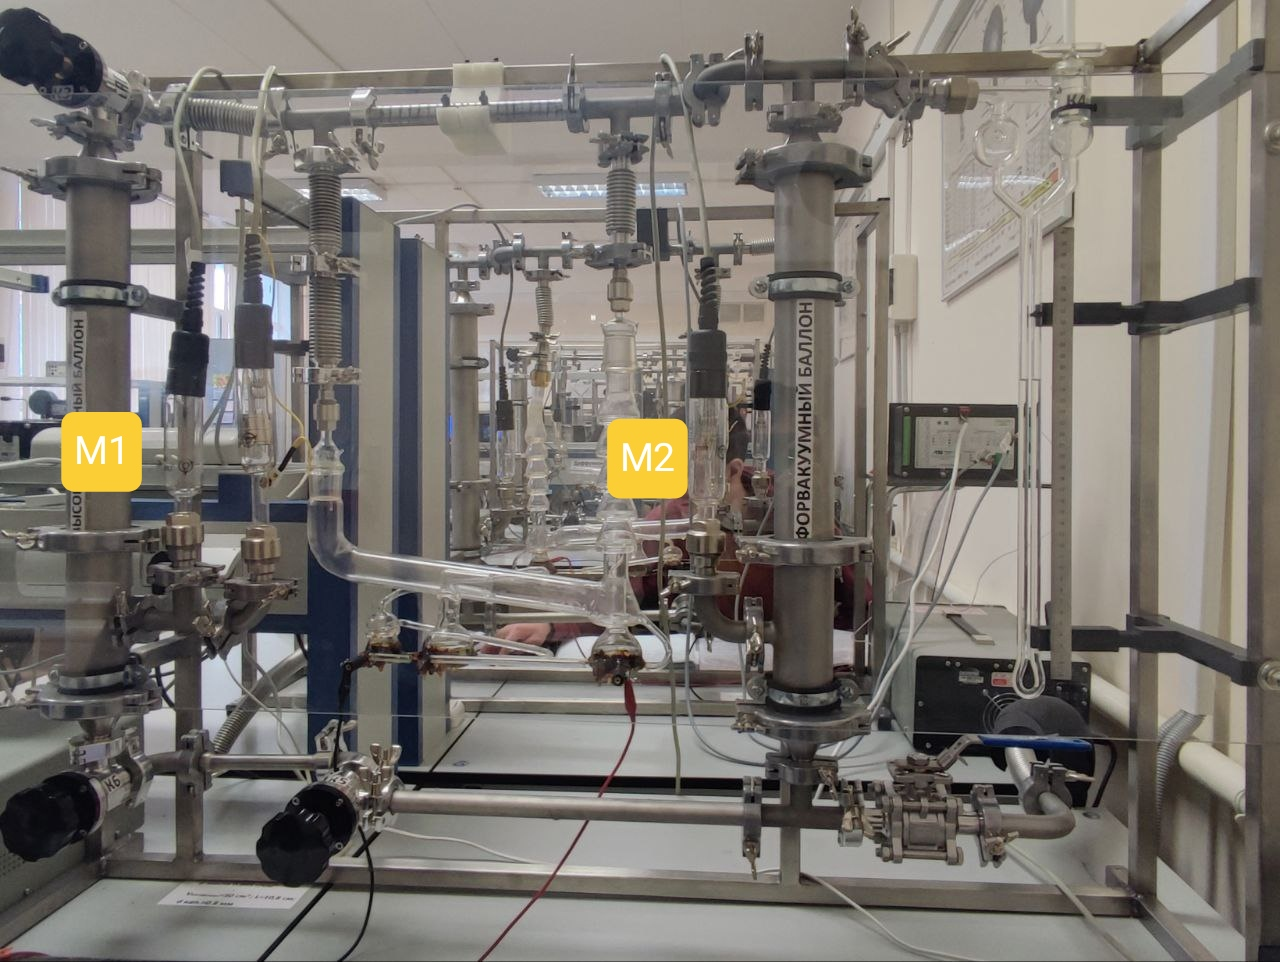
\includegraphics[scale = 0.15]{images/therm.jpg}
    \end{figure}
\end{frame}


\begin{frame}{Ход работы: создание высокого вакуума}
    При достижении давления \(p_{c0}\) закрывается кран \textbf{6},  высоковакуумный баллон остаеться связаным с форвакуумной частью только включенным масляным насосом.
    \begin{figure}[h]
        \centering
        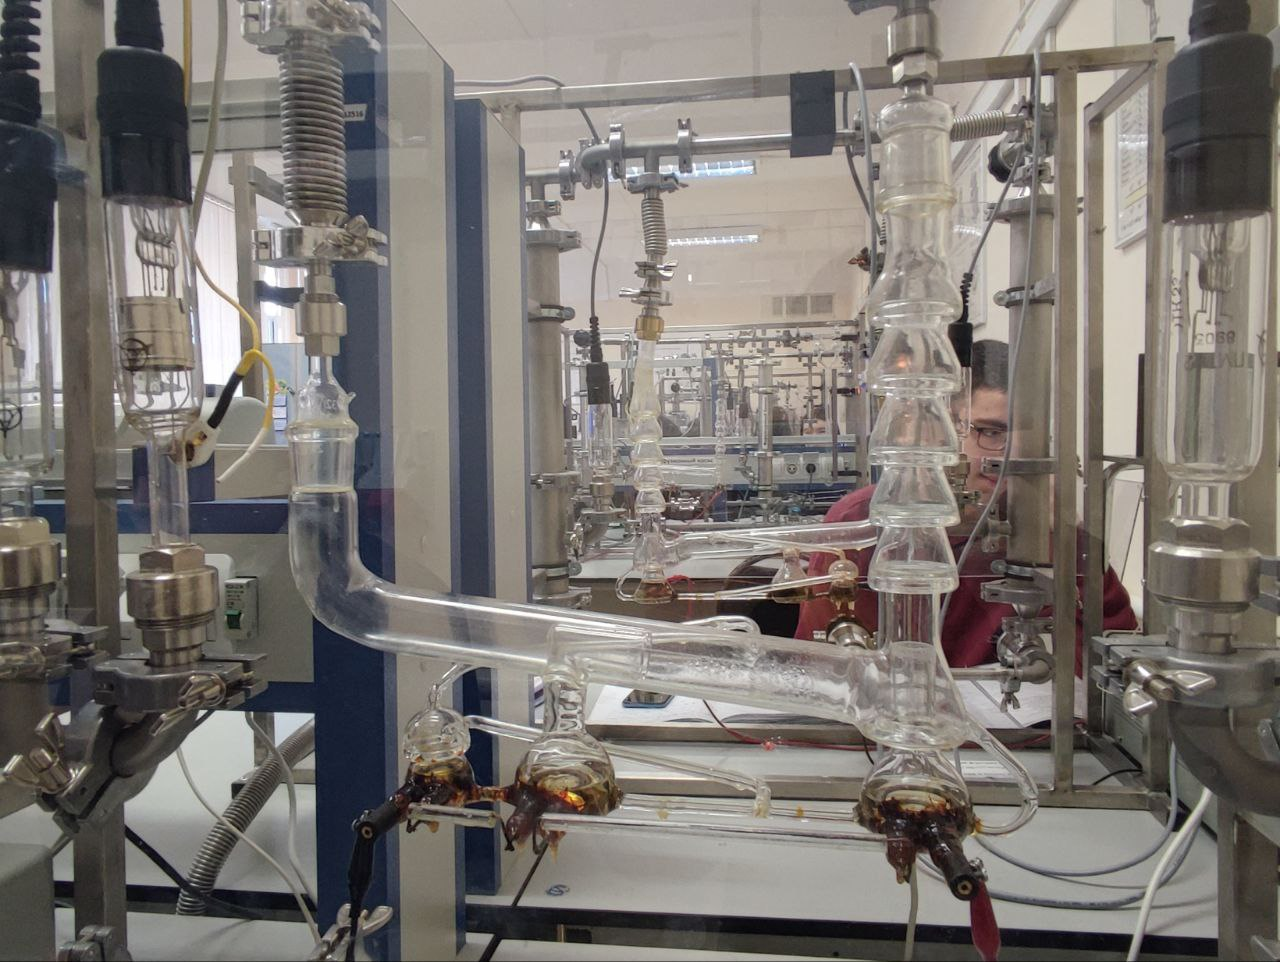
\includegraphics[scale = 0.15]{images/oil_valve.jpg}
    \end{figure}
\end{frame}



\begin{frame}{Ход работы: создание высокого вакуума}
    Когда давление в высоковакуумном баллоне становится ниже \(p_{c1}=1.2 \cdot 10^{-4} \text{ мм.рт.столба }\)
    происходит инициация ионизационного манометра. Можно приступать к измерению скоростей откачки
    \begin{figure}[h]
        \centering
        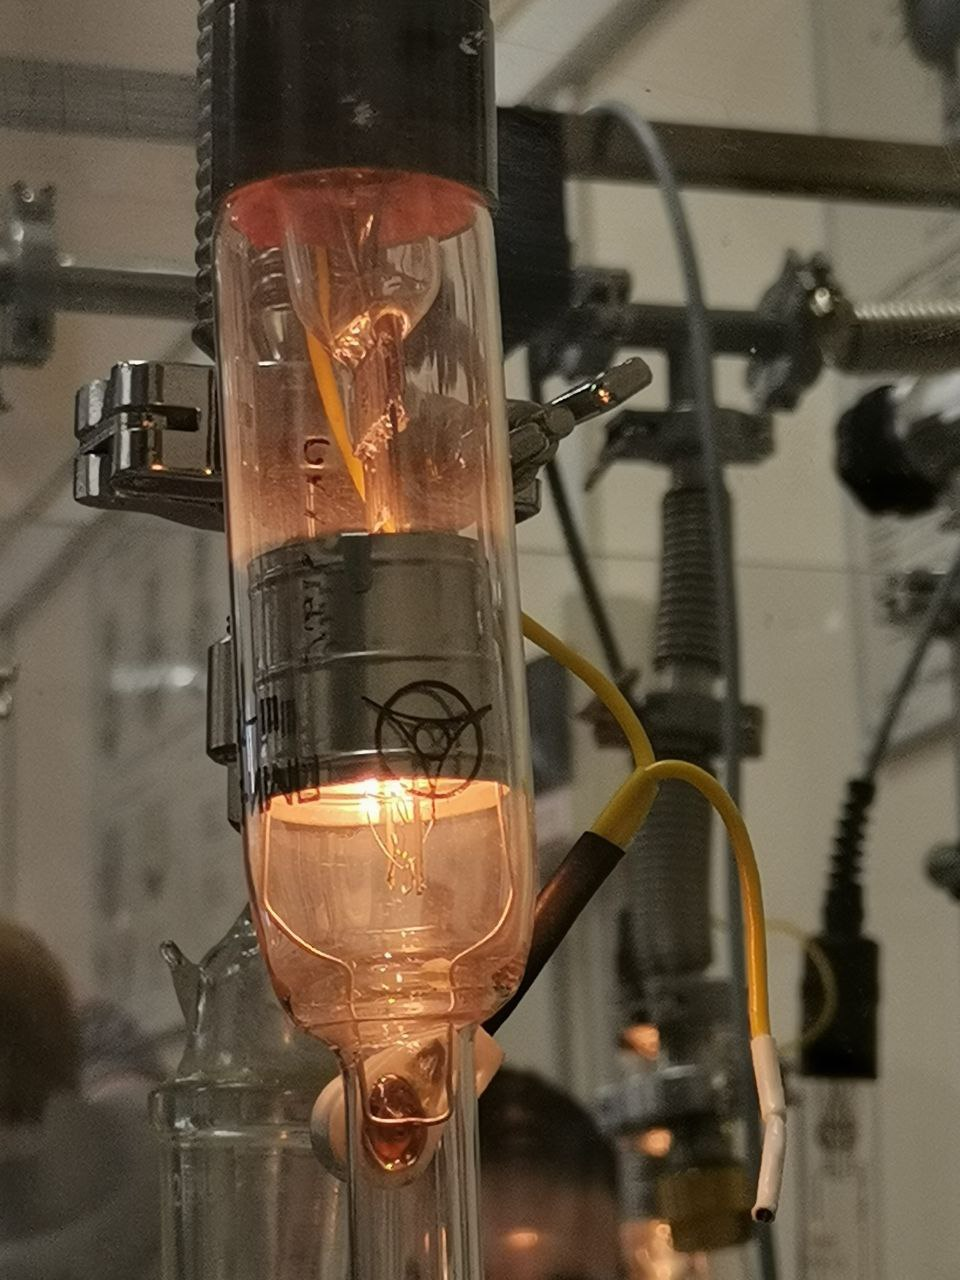
\includegraphics[scale = 0.12]{images/ion.jpg}
    \end{figure}
\end{frame}
\begin{frame}{Измерение скорости откачки газа}
   Основное уравнение откачки газа из высоковакуумного баллона:
   \[-V_hdp = (pW - Q_v - Q_c)dt \ \text{(1)}\]
   При достижении \(p_{lim}\), \text{  } \(\frac{dp}{dt} = 0\), тогда
   \[p_{lim}W = Q_v + Q_c \text{  (2)}\]
   Проинтегрировав (1), получим
   \[p-p_{lim} = p_0-p_{lim}\cdot exp(-\frac{W}{V_h}t)\]
\end{frame}

\begin{frame}{Графики откачки}

\begin{minipage}{.3\textwidth}
    \small Измеряем \(p_\) \\ Открываем кран и с помощью ионизационного манометра получаем зависимость p(t).
    Давление убывает по экспоненциальному закону:
    \[p-p_{lim} = (p_0-p_{lim})exp-\frac{W}{V_h}t,\]
    откуда \(W = -k_1V_h\) \\
    измеренное \(p_{lim} = 5.6\pm0.1 \cdot 10^{-5}\)Торр.
\end{minipage}%
\begin{minipage}{.5\textwidth}
\begin{figure}
    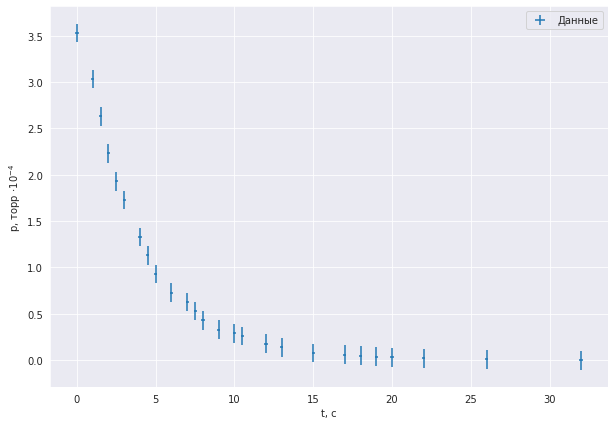
\includegraphics[scale=0.4]{images/exponent_decrease.png}
    \caption{Чистые данные}
    \label{fig:my_label}
\end{figure}
\end{minipage}%

\end{frame}

\begin{frame}{График откачки - Логарифм}
\begin{minipage}{0.3\textwidth}
    Из МНК: \\
    k_1 = -0.23, \text{ откуда:}  \\
    \vspace{5mm}
    W = 41.9 \pm 0.5 \cdot 10^{-2} \frac{\text{л}}{\text{с}}
\end{minipage}%
\begin{minipage}{.5\textwidth}
\begin{figure}
    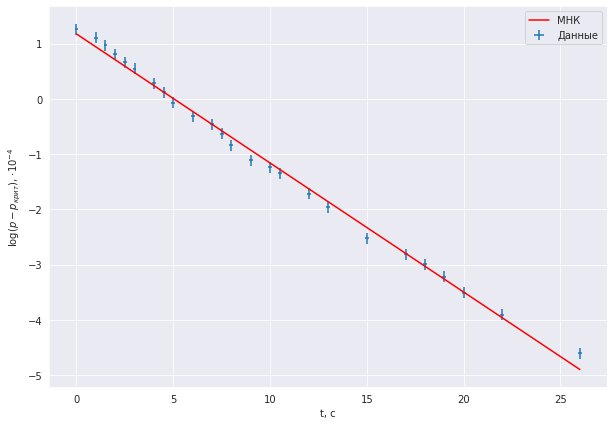
\includegraphics[scale=0.4]{images/log_decrease.png}
    \caption{Логарифм + МНК}
    \label{fig:my_label}
\end{figure}
\end{minipage}%
\end{frame}

\begin{frame}{Графики откачки}

\begin{minipage}{.3\textwidth}
    \small Cнова закрываем кран 3 и получаем зависимость давления от времени (\(p\) от \(t\)) для истечения через микротечи. \\ Здесь насос не возвращает воздух в систему, поэтому \(Q_v = 0\) откуда:
    $$V_hdp = Q_cdt$$
    $$Q_c = 1.82 \pm 0.33 \cdot 10^{-5} $$
    $$k_2 = 0.1 \text{ - коэфф. наклона} \Rightarrow $$
    Q_v = p_{lim}W - Q_c = 0.82 \pm 0.1 \cdot 10^{-5} \frac{\text{Торр}\cdot{\text{Л}}}{\text{с}} 
\end{minipage}%
\begin{minipage}{.5\textwidth}
\begin{figure}
    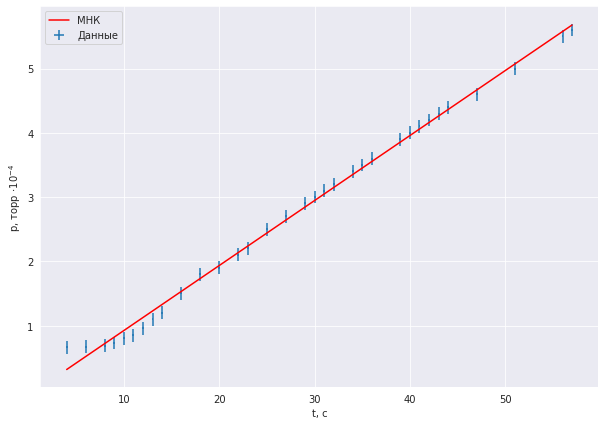
\includegraphics[scale=0.4]{images/micro_current_chart.png}
    \caption{Микротечи}
    \label{fig:my_label}
\end{figure}
\end{minipage}%

\end{frame}

\begin{frame}{Проверка формулы Кнудсена}
    Откроем кран 6, чтобы создать искуственную течь и измерить производительность насоса в предположении формулы Кнудсена.
    \[p_{lim}W=Q\]
    \[p_{const}W=Q+\frac{d(pV)}{dt}\]
    \[\frac{d(pV)}{dt} = \frac{4}{3}r^3\sqrt{\frac{2\pi RT}{\mu}}\frac{p_2-p_1}{l}\]
    Подставив \(p_1 = p_{const}\), \(p_2 = p_f \) - давление в форвакуумной части, получим:
    \[W = \frac{4}{3}
    \frac{r^3}{l}\sqrt{\frac{2\pi RT}{\mu}}\frac{p_f-p_{const}}{p_{const}-p_{lim}}\]
    
\end{frame}

\begin{frame}{Проверка формулы Кнудсена}
   $$  \text{Полученные в эксперименте значения: }$$ $$r = 9 \pm 0.1 \text{мм}, \ l = 63 \pm 1 \text{мм}. $$
    $$ p_{const} = (1.4 \pm 0.1)\cdot 10^{-4} \text{ Торр}, \ p_f = (4.6 \pm 0.1) \cdot 10^{-3} \text{ Торр}, $$ $$\text{Откуда скорость откачки: } $$ $$\(W_{\text{Кнуд}} = (23\pm 3)\cdot 10^{-2}\)\text{ л/с}.$$
\end{frame}


\begin{frame}{Вывод:}
\textbf{Вывод: } В ходе работы был получены высокий вакуум (через 3 стадии) с $$p_{lim} = 6.7  \pm 0.1 \cdot 10^{-5} \text{ торр} $$  расчитаны объемы частей насоса:
$$V_f = 1.82 \pm 0.05 \text{л} \text{ и } V_f = 2.88 \pm 0.05 \text{л}$$
и скорости откачки: $$Q_c = 1.82 \pm 0.33 \cdot 10^{-5} \frac{\text{Торр}\cdot{\text{Л}}}{\text{с}} \text{ и } Q_v = 0.81 \pm 0.1 \cdot 10^{-5} \frac{\text{Торр}\cdot{\text{Л}}}{\text{с}}$$
Скорость откачки экспериментальное и теоретическое:
$$W = 41.9 \pm 0.5 \cdot 10^{-2}  \ \frac{\text{Л}}{\text{с}} \  W_{\text{Кнуд}} = 23 \pm 3 \cdot 10^{-2} \ \frac{\text{Л}}{\text{с}}$$

\end{frame}

\begin{frame}{Исходники:}
\begin{itemize}
    \item \href{https://github.com/hK04/LabWorksSecondSem/tree/main/Vacuum}{Github с обработкой данных и .tex презентацией}
    \item \href{https://docs.google.com/spreadsheets/d/12a_L3i0lo_ZkRGvZ3DAzGaIObqutBBe5veAsxOcPjug/edit?ouid=115306472035042428210&usp=sheets_home&ths=true}{Снятые данные}
\end{itemize}
\end{frame}

%\begin{frame}{Приложение:}
%    \begin{figure}
%        \centering
%        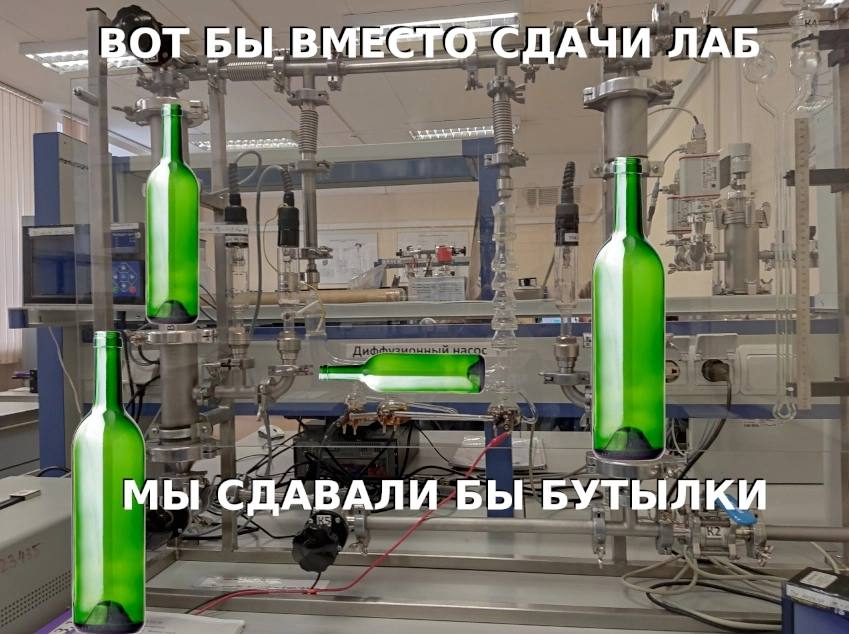
\includegraphics[scale=0.4]{images/photo_2023-02-18_00-12-39.jpg}
%        \caption{Caption}
%        \label{fig:my_label}
%    \end{figure}
%\end{frame}
